\section{Resultados e Discussão}
\label{chap:resultados}

A investigação empírica do Terceiro Trabalho Computacional permitiu confrontar o desempenho de modelos probabilísticos e baseados em protótipos em diferentes espaços de representação. A análise a seguir detalha o impacto da redução de dimensionalidade e a eficácia das arquiteturas de decisão implementadas.

\subsection{Análise de Redução de Dimensionalidade (PCA)}
A aplicação do PCA sobre os 24 sensores revelou uma estrutura de dados com variância distribuída, conforme ilustrado na Figura~\ref{fig:pca_plots}. O gráfico de variância individual (\textit{Scree Plot}) indica que não há um domínio absoluto de poucas componentes, o que é coerente com a análise de condicionamento do TC2, onde as matrizes apresentaram posto completo.

\begin{figure}[h]
    \centering
    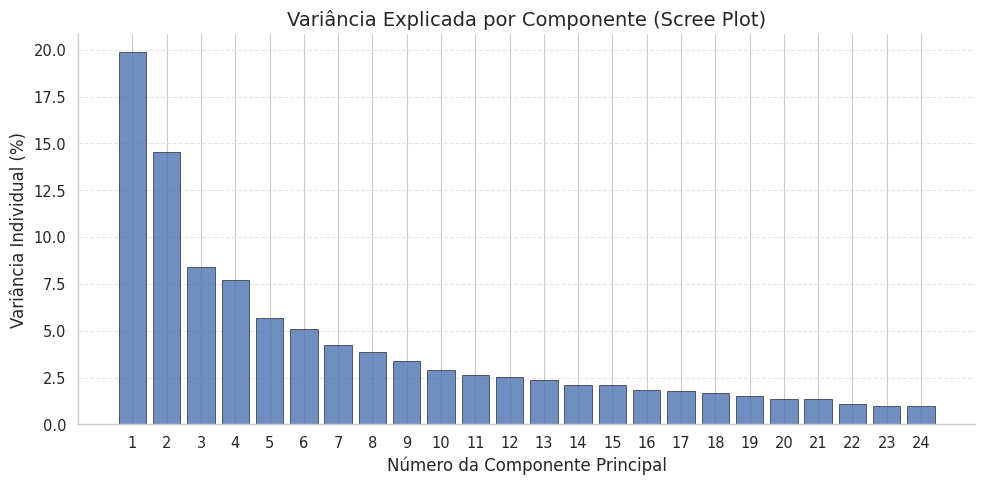
\includegraphics[width=0.48\textwidth]{figuras/variancia_individual.png}
    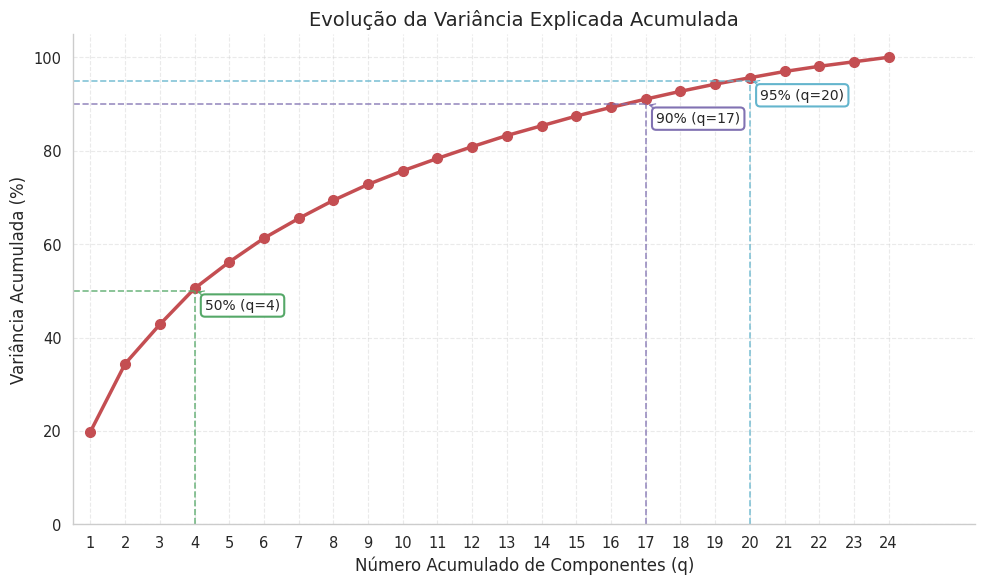
\includegraphics[width=0.48\textwidth]{figuras/pca_variancia_acumulada.png}
    \caption{À esquerda, variância explicada individual por componente. À direita, variância acumulada evidenciando os pontos de retenção de 50\%, 90\% e 95\%.}
    \label{fig:pca_plots}
\end{figure}

Para reter $95\%$ da variância original, foram necessárias $q=20$ componentes principais. Esta observação confirma que, apesar da redundância espacial dos sensores, a informação útil está espalhada pelo espectro de atributos. Para os experimentos oficiais de classificação com redução, optou-se por $q=18$ componentes, ponto onde a curva de variância começa a estabilizar, oferecendo um bom compromisso entre compressão e preservação de sinal.

\subsection{Desempenho dos Classificadores: CQG vs DMP}
A Tabela~\ref{tab:acuracia_final} apresenta a acurácia média obtida em 100 rodadas de Monte Carlo. O Classificador Quadrático Gaussiano (CQG) demonstrou uma estabilidade notável, mantendo o desempenho mesmo após a redução para 18 dimensões ($67,76\%$ vs $68,14\%$). Este resultado justifica a eficácia do PCA em remover ruído sem comprometer a estrutura das densidades Gaussianas.

\begin{table}[h]
\centering
\caption{Comparativo de Acurácia Média $\pm$ Desvio Padrão (100 rodadas).}
\label{tab:acuracia_final}
\resizebox{\columnwidth}{!}{%
\begin{tabular}{l|cc}
\toprule
\textbf{Classificador} & \textbf{Espaço Original (24D)} & \textbf{Espaço Reduzido (PCA - 18D)} \\
\midrule
CQG (Probabilístico) & $0,6814 \pm 0,0114$ & $0,6776 \pm 0,0114$ \\
DMP (Multi-Protótipo) & $\mathbf{0,7220 \pm 0,0640}$ & $0,6386 \pm 0,1016$ \\
\bottomrule
\end{tabular}%
}
\end{table}

O modelo DMP Multi-Protótipo obteve a maior acurácia absoluta no espaço original ($72,20\%$), evidenciando que a partição de Voronoi flexível (com múltiplos centros de massa por classe) captura melhor a geometria não-linear dos dados de navegação. Contudo, o DMP apresentou maior sensibilidade ao PCA, com queda de desempenho e aumento do desvio padrão, sugerindo que a redução linear pode ter fundido regiões de decisão que eram separáveis via protótipos locais no espaço original.

\subsection{Validação de Clusters e Superfícies de Decisão}
A escolha automática do número de protótipos ($K$) para o DMP via votação de índices (DB, CH, Dunn, Sil, I-Index, Ball-Hall) revelou que a classe \textit{Slight-Left-Turn} exigiu o maior número de protótipos ($K=36$), enquanto outras classes foram bem representadas com menos centros. A Figura~\ref{fig:decision_boundaries} visualiza as regiões de decisão projetadas em 2D. Nota-se que o CQG gera fronteiras suaves e parabólicas, enquanto o DMP cria uma fronteira "facetada" e complexa, capaz de se adaptar a \textit{clusters} multimodais.

\begin{figure}[h]
    \centering
    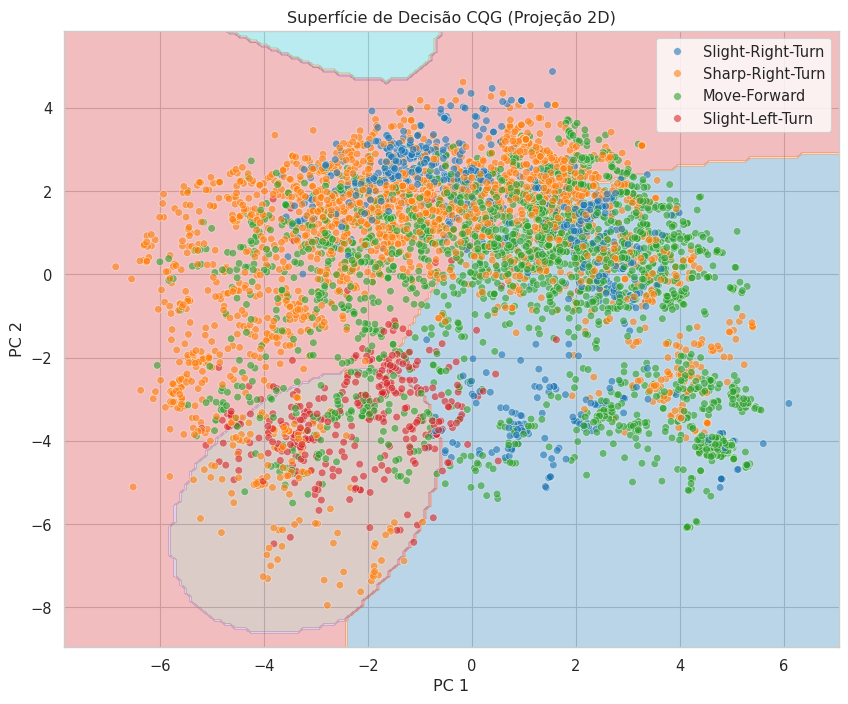
\includegraphics[width=0.48\textwidth]{figuras/superficie_decisao_cqg.png}
    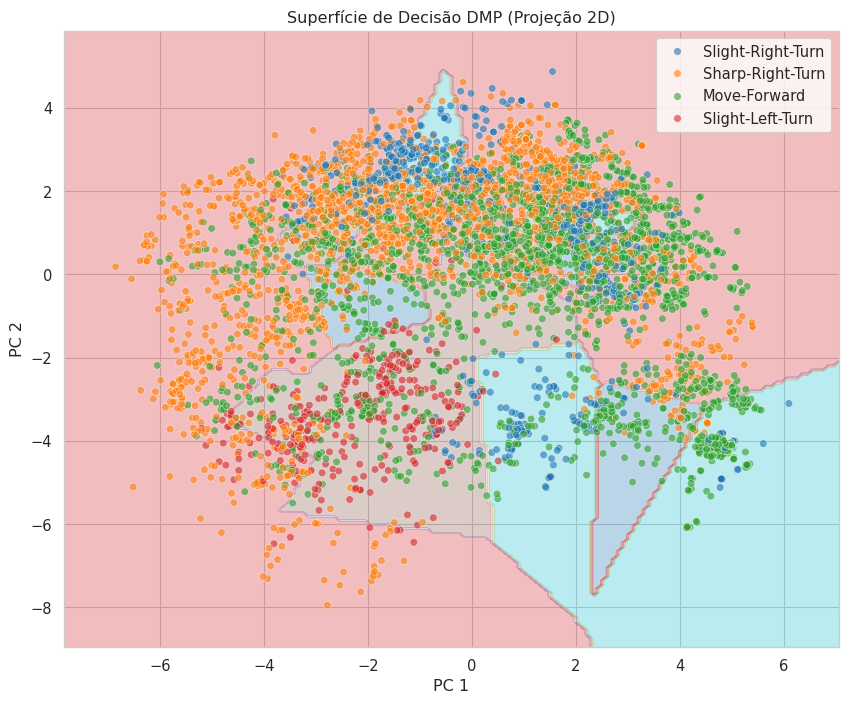
\includegraphics[width=0.48\textwidth]{figuras/superficie_decisao_dmp.png}
    \caption{Superfícies de decisão projetadas nas duas primeiras componentes principais (PCA). À esquerda o CQG e à direita o DMP Multi-Protótipo.}
    \label{fig:decision_boundaries}
\end{figure}

Por fim, a análise da matriz de confusão (Figura~\ref{fig:confusion}) indicou que a classe minoritária \textit{Slight-Right-Turn} sofre o maior viés, sendo frequentemente confundida com a movimentação frontal. Este comportamento ressalta a necessidade de considerar o desbalanceamento de classes em futuras iterações do sistema.

\begin{figure}[h]
    \centering
    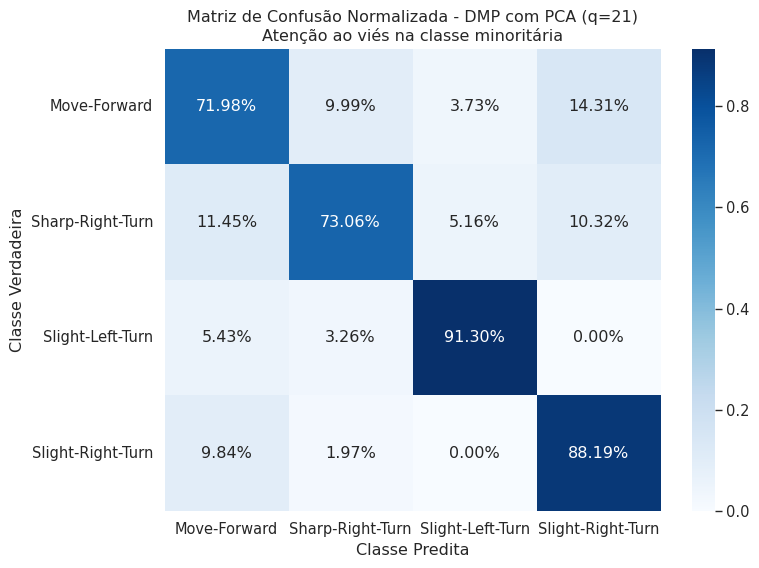
\includegraphics[width=0.6\textwidth]{figuras/matriz_confusao_normalizada.png}
    \caption{Matriz de Confusão Normalizada para o DMP com PCA. Valores na diagonal representam o \textit{Recall} por classe.}
    \label{fig:confusion}
\end{figure}
